\documentclass[11pt,a4paper]{article}
\usepackage[utf8]{inputenc}
\usepackage[spanish,es-noquoting]{babel}
\usepackage{amsmath,amsfonts,amssymb}
\usepackage{geometry}
\geometry{top=2.3cm, bottom=2.3cm, left=2.3cm, right=2.3cm}
\usepackage{hyperref}
\usepackage{booktabs}
\usepackage{tabularx}
\usepackage{xcolor}
\usepackage{tcolorbox}
\tcbuselibrary{skins,breakable}
\usepackage{enumitem}
\setlist{nosep, topsep=3pt, partopsep=0pt}
\usepackage{graphicx}
\usepackage{tikz}
\usetikzlibrary{shapes.geometric, arrows.meta, positioning, calc, fit}

\raggedbottom

% ---------------------------------------------------------
% PALETA INSTITUCIONAL Y DEFINICIÓN DE COLORES
% ---------------------------------------------------------
\definecolor{primary}{RGB}{0, 51, 102}      % Azul Institucional Externado (#003366)
\definecolor{secondary}{RGB}{232, 119, 34}  % Naranja Externado (#E87722)
\definecolor{accent}{RGB}{0, 114, 206}      % Azul Tecnológico
\definecolor{darkgray}{RGB}{40, 40, 40}
\definecolor{lightgray}{RGB}{245, 247, 250}
\definecolor{bordergray}{RGB}{205, 215, 225}
\definecolor{success}{RGB}{46, 125, 50}     % Verde Validación (#2E7D32)
\definecolor{warning}{RGB}{217, 119, 6}     % Ámbar Ajuste Metodológico (#D97706)
\definecolor{danger}{RGB}{192, 57, 43}      % Rojo Crítico (#C0392B)

\hypersetup{
    colorlinks=true,
    linkcolor=primary,
    citecolor=secondary,
    urlcolor=accent,
    pdftitle={Entrega No. 3 - Trabajo de Campo 2 con Clientes - Wheels Externado}
}

% ---------------------------------------------------------
% ESTILOS DE CAJAS PERSONALIZADAS
% ---------------------------------------------------------
\newtcolorbox{externadobox}[2][]{
    enhanced,
    colback=lightgray,
    colframe=primary,
    coltitle=white,
    fonttitle=\bfseries\sffamily,
    title={#2},
    sharp corners=south,
    arc=3.5mm,
    boxrule=1.1pt,
    left=3.5mm, right=3.5mm, top=2.5mm, bottom=2.5mm,
    #1
}

\newtcolorbox{evidencebox}[2][]{
    enhanced,
    colback=secondary!6,
    colframe=secondary,
    coltitle=white,
    fonttitle=\bfseries\sffamily,
    title={#2},
    arc=3mm,
    boxrule=1pt,
    left=3.5mm, right=3.5mm, top=2.5mm, bottom=2.5mm,
    #1
}

\newtcolorbox{kbibox}[2][]{
    enhanced,
    colback=success!6,
    colframe=success,
    coltitle=white,
    fonttitle=\bfseries\sffamily,
    title={#2},
    arc=3mm,
    boxrule=1pt,
    left=3.5mm, right=3.5mm, top=2.5mm, bottom=2.5mm,
    #1
}

\newtcolorbox{warningbox}[2][]{
    enhanced,
    colback=warning!6,
    colframe=warning,
    coltitle=white,
    fonttitle=\bfseries\sffamily,
    title={#2},
    arc=3mm,
    boxrule=1pt,
    left=3.5mm, right=3.5mm, top=2.5mm, bottom=2.5mm,
    #1
}

\begin{document}

% ---------------------------------------------------------
% PORTADA INSTITUCIONAL
% ---------------------------------------------------------
\begin{titlepage}
    \centering
    \vspace*{0.5cm}
    {\Huge \textbf{\color{primary} UNIVERSIDAD EXTERNADO DE COLOMBIA}}\\[0.3cm]
    {\Large \textbf{\color{secondary} PREGRADO EN CIENCIA DE DATOS --- EMPRENDIMIENTO}}\\[1.5cm]
    
    \rule{\linewidth}{0.8mm}\\[0.4cm]
    {\Huge \textbf{ENTREGA NO. 3: TRABAJO DE CAMPO 2}}\\[0.3cm]
    {\Large \textbf{Customer Discovery con Clientes y Validaci\'on de Hip\'otesis:\\Entrevistas Semiestructuradas, Evaluaci\'on de Concepto y Dise\~no de Canales}}\\[0.4cm]
    \rule{\linewidth}{0.8mm}\\[1.2cm]
    
    \begin{tcolorbox}[colback=primary!5,colframe=primary,arc=4mm,boxrule=1.5pt]
        \centering \huge \color{primary}
        \textbf{Wheels Externado} \\[0.2cm]
        \large \color{darkgray}
        \textit{Plataforma Inteligente de Carpooling Universitario y Movilidad Sostenible}
    \end{tcolorbox}
    
    \vspace{1.8cm}
    
    \begin{minipage}{0.85\textwidth}
        \centering \large
        \textbf{Equipo No. 5:}\\[0.25cm]
        \textbf{Juli\'an Duarte} --- \texttt{julian.duarte@externado.edu.co}\\[0.15cm]
        \textbf{Tom\'as Rinc\'on} --- \texttt{tomas.rincon@externado.edu.co}\\[0.15cm]
        \textbf{Sebasti\'an Cuervo} --- \texttt{sebastian.cuervo@externado.edu.co}\\[0.6cm]
        \textbf{Docente Titular:} C\'atedra de Emprendimiento e Innovaci\'on\\[0.15cm]
        \textbf{Programa Acad\'emico:} Pregrado en Ciencia de Datos\\[0.15cm]
        \textbf{Facultad:} Ingenier\'ia y Tecnolog\'ias de la Informaci\'on
    \end{minipage}
    
    \vfill
    {\large \textbf{Bogot\'a D.C., Colombia --- Octubre de 2026}}
\end{titlepage}

\tableofcontents
\newpage

% =========================================================
% PARTE I: INFORME EJECUTIVO Y VALIDACIÓN DE CAMPO
% =========================================================
\section{Punto de Partida, Segmento y Contexto del Proyecto}

\subsection{El Negocio en una Frase}
\begin{externadobox}{Definici\'on Estrat\'egica del Emprendimiento}
\textbf{Wheels Externado} es una plataforma m\'ovil inteligente de carpooling hiperlocal que conecta a estudiantes y docentes de la Universidad Externado de Colombia que viajan solos en autom\'ovil particular con compa\~neros de su misma ruta y facultad, garantizando reserva anticipada sin la loter\'ia de mensajes en WhatsApp, validaci\'on institucional obligatoria con credencial \texttt{@uexternado.edu.co}, liquidaci\'on digital instant\'anea a billeteras m\'oviles y rutas seguras exclusivas para mujeres.
\end{externadobox}

\subsection{Contexto del Pivote Metodol\'ogico}
El proyecto inicial del equipo, \textit{StatCredit AI} (modelo predictivo de score crediticio alternativo para trabajadores informales), fue sometido a evaluaci\'on cr\'itica tras el Trabajo de Campo 1. Dicho an\'alisis arroj\'o barreras estructurales insalvables para una etapa temprana: alta regulaci\'on de la Superintendencia Financiera de Colombia (SFC), rigidez en la integraci\'on con bureaus tradicionales (Datacr\'edito, TransUnion), y un ciclo de ventas B2B superior a 9 meses que imped\'ia la iteraci\'on \'agil con usuarios finales.

Ante este panorama, el equipo aplic\'o el principio de \textit{Customer Discovery} de Steve Blank: \guillemotleft salir del edificio\guillemotright\ para resolver un dolor cr\'itico, diario, recurrente y accesible en nuestro propio entorno. La Universidad Externado de Colombia, ubicada en los cerros orientales del barrio La Candelaria, presenta un aislamiento geogr\'afico severo y una oferta deficitaria de transporte p\'ublico masivo:
\begin{itemize}[leftmargin=*]
    \item \textbf{Saturaci\'on del Transporte P\'ublico:} Los estudiantes procedentes de la periferia urbana (Suba, Calle 80, Bosa, Kennedy) y municipios sabaneros (Facatativ\'a, Soacha) padecen trayectos de 90 a 150 minutos por sentido en rutas de TransMilenio y SITP saturadas, con transbordos forzados y caminatas empinadas no iluminadas hacia el campus.
    \item \textbf{Costo de Alternativas Privadas:} El uso de taxis o plataformas de ride-hailing tradicionales (Uber, DiDi, InDrive) representa un gasto de \$25.000 a \$45.000 COP por viaje, un costo astron\'omico e inviable para el presupuesto semanal de un estudiante universitario.
    \item \textbf{Ineficiencia de los Chats Informales de WhatsApp:} Existen actualmente al menos 4 macrogrupos de WhatsApp de carpooling estudiantil (\textit{Wheels Externado}). No obstante, operan como un canal an\'arquico: entre 400 y 600 mensajes diarios sepultan la oferta de rutas, no existen reservas garantizadas, la impuntualidad y las cancelaciones a \'ultima hora (\textit{ghosting}) alcanzan el 35\%, y no hay verificaci\'on confiable sobre qui\'en aborda o conduce.
\end{itemize}

\subsection{El Segmento Objetivo: Plataforma de Dos Lados (\textit{Two-Sided Market})}
Siguiendo la disciplina de Bill Aulet (2017, Paso 1), el mercado de Wheels Externado est\'a compuesto por dos actores interdependientes que deben ser alineados simult\'aneamente:
\begin{enumerate}[leftmargin=*]
    \item \textbf{La Demanda (Pasajeros):} Estudiantes regulares de pregrado y posgrado residentes en corredores perif\'ericos (a m\'as de 60 minutos de viaje) que carecen de autom\'ovil y buscan un viaje r\'apido, seguro y asequible.
    \item \textbf{La Oferta (Conductores):} Estudiantes que se desplazan diariamente al campus en autom\'ovil propio con hasta 4 sillas desocupadas, y que sufren el alto costo del parqueadero institucional (\$22.000 COP diarios) y el consumo de gasolina.
\end{enumerate}

% ---------------------------------------------------------
\section{Dise\~no Metodol\'ogico de la Investigaci\'on de Campo}

\subsection{Objetivos de la Investigaci\'on}
\textbf{Objetivo General:} Validar emp\'iricamente con 12 estudiantes activos de la Universidad Externado de Colombia (8 pasajeros y 4 conductores de carpooling) c\'omo gestionan hoy sus traslados al campus, qui\'en y c\'omo decide el pago de la tarifa, qu\'e canales utilizan para conectarse y qu\'e relaci\'on de confianza esperan de una plataforma institucional, mediante entrevistas semiestructuradas realizadas entre el 17 y el 30 de octubre de 2026, con el fin de fundamentar la decisi\'on estrat\'egica de perseverar, ajustar o pivotar el prototipo antes de las pruebas de usuario del Trabajo de Campo 3.

\textbf{Objetivos Espec\'ificos:}
\begin{itemize}[leftmargin=*]
    \item \textbf{OE1 (Problema y Costos):} Cuantificar la frecuencia, la severidad de los dolores cr\'iticos y los costos en tiempo y dinero que afrontan pasajeros y conductores en sus desplazamientos habituales hacia el campus.
    \item \textbf{OE2 (Unidad de Toma de Decisi\'on y Canales):} Determinar qui\'en usa, qui\'en financia, qui\'en recomienda y qui\'en puede vetar la decisi\'on de tomar un viaje compartido, identificando los canales de adquisici\'on m\'as eficaces en el campus.
    \item \textbf{OE3 (Concepto, Relaci\'on y Compromisos):} Evaluar la receptividad de los usuarios ante el concepto funcional de una aplicaci\'on institucional verificada, recolectando compromisos verificables para las pruebas del prototipo interactivo (Campo 3).
\end{itemize}

\subsection{Hip\'otesis de Investigaci\'on y Criterios de Aceptaci\'on \textit{Ex Ante}}
Antes de abordar al primer informante, el equipo formaliz\'o tres hip\'otesis seg\'un la formulaci\'on de Steve Blank y fij\'o criterios objetivos y medibles de \'exito:

\begin{table}[!htbp]
\centering
\small
\renewcommand{\arraystretch}{1.2}
\begin{tabularx}{\textwidth}{p{2.8cm}Xp{4.2cm}}
\toprule
\textbf{Hip\'otesis} & \textbf{Formulaci\'on \textit{Ex Ante}} & \textbf{Criterio de Aceptaci\'on} \\
\midrule
\textbf{H1 (Problema)} & Creemos que los estudiantes y conductores del Externado viven el transporte diario como un dolor cr\'itico de alta prioridad y consideran a los grupos de WhatsApp ineficientes e inseguros. & Se valida si al menos \textbf{10 de 12} entrevistados ($\ge 83,3\%$) lo describen con ejemplos concretos de su rutina. \\
\midrule
\textbf{H2 (Compra)} & Creemos que el pasajero decide y paga individualmente el servicio de carpooling, que la tarifa de referencia es de \$6.000 COP y que estar\'ia dispuesto a pagar una prima adicional por certeza de cupo y seguridad, mientras el conductor busca amortizar parqueadero y gasolina. & Se valida si al menos \textbf{9 de 12} entrevistados ($\ge 75,0\%$) confirman la tarifa base de \$6.000 y autonom\'ia en el pago. \\
\midrule
\textbf{H3 (Relaci\'on)} & Creemos que el usuario adoptar\'ia una plataforma institucional verificada (\texttt{@uexternado.edu.co}) que garantice cupo fijo, reputaci\'on y pago digital, y que otorgar\'a un compromiso formal para probar el prototipo en el Campo 3. & Se valida si al menos \textbf{8 de 12} nombran estas condiciones y al menos \textbf{4 de 12} aceptan participar en la prueba de usuario. \\
\bottomrule
\end{tabularx}
\caption{Matriz de hip\'otesis y criterios de aceptaci\'on del Trabajo de Campo 2.}
\label{tab:hipotesis}
\end{table}

\subsection{Poblaci\'on, Criterios de Inclusi\'on y Exclusi\'on}
\begin{itemize}[leftmargin=*]
    \item \textbf{Poblaci\'on Objetivo:} Estudiantes regulares de pregrado del Externado que asisten presencialmente a clases en el campus y deben recorrer distancias medias o largas dentro de Bogot\'a o la Sabana.
    \item \textbf{Criterios de Inclusi\'on:} (1) Matr\'icula acad\'emica activa en el Externado; (2) Uso o prestaci\'on de servicio de carpooling al menos 1 vez por semana; (3) Trayecto de origen o destino en corredores perif\'ericos; (4) Disponibilidad de 30 a 40 minutos para la entrevista semiestructurada.
    \item \textbf{Criterios de Exclusi\'on:} Amigos \'intimos, familiares cercanos o compa\~neros de trabajo directo del equipo (para evitar el sesgo de deseabilidad social o cortes\'ia); expertos entrevistados en el Campo 1; personas sin v\'inculo con el campus.
\end{itemize}

\subsection{Embudo de Reclutamiento}
El proceso de reclutamiento se desarroll\'o en dos fases cronol\'ogicas:
\begin{enumerate}
    \item \textbf{Fase Inicial (17 al 21 de octubre):} Se contactaron 15 estudiantes v\'ia mensaje directo en los chats comunitarios de WhatsApp de Wheels. Respondieron 10, de los cuales 8 cumplieron los filtros y completaron la entrevista (E1 a E8).
    \item \textbf{Fase Complementaria (28 al 30 de octubre):} Para robustecer la muestra con conductores adicionales y someter a prueba la hoja de concepto visual, se contactaron 10 candidatos adicionales. Respondieron 6, de los cuales 4 fueron aprobados y entrevistados (E9 a E12).
\end{enumerate}

\begin{externadobox}{Embudo Consolidado de Investigaci\'on de Campo}
\centering
\textbf{25 Candidatos Contactados} $\;\longrightarrow\;$ \textbf{16 Respondieron (64\%)} $\;\longrightarrow\;$ \textbf{12 Filtros Superados (75\%)} $\;\longrightarrow\;$ \textbf{12 Entrevistas Efectivas (100\%)}
\end{externadobox}

% ---------------------------------------------------------
\section{Caracterizaci\'on de Arquetipos de Cliente (User Personas)}

\subsection{User Persona 1: Valentina Duarte (Demanda --- Pasajera Beachhead)}
\begin{evidencebox}{Arquetipo de Pasajera: Valentina Duarte}
\textbf{Datos Demogr\'aficos:} 21 a\~nos, estudiante de 6.\textsuperscript{to} semestre de Derecho, residente en el barrio Timiza (Kennedy). Carece de veh\'iculo propio.\\
\textbf{Comportamiento Diario:} Clases de 7:00 a.m. Debe despertarse a las 4:30 a.m. para abordar el TransMilenio en el Portal Am\'ericas; sufre aglomeraciones, retrasos frecuentes y caminatas solitarias en La Candelaria.\\
\textbf{Dolores Cr\'iticos:} Inseguridad percibida al esperar transporte p\'ublico de noche; estr\'es cr\'onico por la \guillemotleft loter\'ia de WhatsApp\guillemotright\ (enviar \guillemotleft yo\guillemotright\ y no alcanzar cupo); miedo a viajar con desconocidos sin filtro institucional.\\
\textbf{Alternativa Actual:} Paga \$6.000 COP en chats informales de WhatsApp cuando logra cupo; de lo contrario, gasta hasta \$30.000 COP en Uber por urgencia de parciales.\\
\textbf{Criterio Clave de Decisi\'on:} Reserva con cupo asegurado la noche anterior y filtro exclusivo de \guillemotleft Solo Chicas\guillemotright.
\end{evidencebox}

\subsection{User Persona 2: Mateo G\'omez (Oferta --- Conductor Beachhead)}
\begin{evidencebox}{Arquetipo de Conductor: Mateo G\'omez}
\textbf{Datos Demogr\'aficos:} 22 a\~nos, estudiante de 7.\textsuperscript{mo} semestre de Econom\'ia, residente en Cedritos (Usaqu\'en). Propietario de un autom\'ovil sedan modelo 2018.\\
\textbf{Comportamiento Diario:} Desciende por la Autopista Norte y Circunvalar solo en su veh\'iculo hacia el campus. Parquea en el parqueadero oficial del Externado.\\
\textbf{Dolores Cr\'iticos:} Gasto mensual desbordado en parqueadero institucional (\$22.000 COP diarios $\approx$ \$440.000 COP/mes) y gasolina; cancelaciones intempestivas de pasajeros a 5 minutos de la salida (\textit{ghosting}), lo que le deja cupos vac\'ios que no puede recuperar.\\
\textbf{Alternativa Actual:} Publica manualmente en 4 chats de WhatsApp cada tarde; cobra \$6.000 COP por cupo, pero gasta hasta 40 minutos coordinando transferencias por Nequi o buscando cambio en efectivo.\\
\textbf{Criterio Clave de Decisi\'on:} Liquidaci\'on digital centralizada inmediata y penalizaci\'on econ\'omica autom\'atica a los pasajeros que cancelen tarde.
\end{evidencebox}

% ---------------------------------------------------------
\section{An\'alisis Cualitativo y Cuantitativo de Hallazgos Emp\'iricos}

\subsection{Tema 1: Vivencia del Problema y Frecuencia de los Dolores}
Los resultados de las 12 entrevistas corroboran que el transporte diario es una de las mayores fuentes de estr\'es, fatiga y merma en la calidad de vida de los externadistas. Se identificaron 4 dolores primarios compartidos:

\begin{table}[!htbp]
\centering
\small
\renewcommand{\arraystretch}{1.2}
\begin{tabularx}{\textwidth}{>{\raggedright\arraybackslash\bfseries}p{4.8cm}ccX}
\toprule
Dolor Identificado en Campo & Frecuencia & Proporci\'on & Informantes que lo Reportan \\
\midrule
1. Desorden e ineficiencia en WhatsApp (mensajes sepultados, sin filtros de ruta) & 8 / 12 & 66,7\% & E1, E2, E3, E5, E7, E9, E10, E11 \\
2. Inseguridad percibida o falta de informaci\'on de los ocupantes & 7 / 12 & 58,3\% & E1, E4, E5, E8, E9, E10, E11 \\
3. Incumplimiento de la contraparte (\textit{ghosting} y cancelaci\'on tard\'ia) & 6 / 12 & 50,0\% & E2, E4, E5, E7, E11, E12 \\
4. Incertidumbre horaria y descalce en la hora de abordaje & 4 / 12 & 33,3\% & E1, E2, E4, E6 \\
\bottomrule
\end{tabularx}
\caption{Distribuci\'on de frecuencias de los dolores cr\'iticos en la muestra validada.}
\label{tab:frecuencias_dolor}
\end{table}

\begin{evidencebox}{Evidencia Textual de los Entrevistados sobre el Problema}
\begin{itemize}[leftmargin=*]
    \item \textbf{E1 (Pasajero, Derecho):} \textit{\guillemotleft Entrar a los grupos de WhatsApp a las 6:00 p.m. es una loter\'ia estresante. Si el conductor escribe una ruta por la 80, hay 15 personas respondiendo 'yo' al mismo segundo. Si no est\'as pegado a la pantalla, te quedas sin puesto y te toca mamarte dos horas de TransMilenio al d\'ia siguiente.\guillemotright}
    \item \textbf{E5 (Conductor, Econom\'ia):} \textit{\guillemotleft Publico que salgo de Cedritos a las 6:30 a.m. Me reservan tres compa\~neros por chat. A las 6:25 a.m., dos me escriben que se quedaron dormidos. Me dejan colgado con los puestos vac\'ios, pierdo \$12.000 COP y llego al campus con la misma rabia de pagar el parqueadero solo.\guillemotright}
    \item \textbf{E6 (Pasajero, Derecho --- procede de Soacha):} \textit{\guillemotleft Duermo apenas cuatro horas al d\'ia por culpa del transporte. Si no consigo un compa\~nero que me acerque en carro, el trayecto en bus intermunicipal y TransMilenio me toma m\'as de dos horas y media de ida y otras dos de vuelta.\guillemotright}
    \item \textbf{E8 (Pasajero, Comunicaci\'on Social):} \textit{\guillemotleft Una vez me mont\'e en un carro de un grupo informal donde al conductor se le notaba aliento alcoh\'olico y manejaba como un loco por la Circunvalar. No ten\'ia c\'omo denunciarlo ni sab\'ia a qui\'en quejarme porque en WhatsApp no hay registros de nada.\guillemotright}
    \item \textbf{E10 (Pasajero, Ingenier\'ia Industrial):} \textit{\guillemotleft Leer 400 mensajes para encontrar un viaje que coincida con mi horario es perder la ma\~nana. Necesitamos filtros autom\'aticos por corredores.\guillemotright}
\end{itemize}
\end{evidencebox}

\subsection{Tema 2: Alternativas Actuales y Estructura de Costos}
Los informantes recurren a una combinaci\'on heterog\'enea y costosa de soluciones temporales:
\begin{itemize}[leftmargin=*]
    \item \textbf{Grupos de WhatsApp Comunitarios (11 de 12 usuarios):} Es la alternativa dominante por defecto. Sin embargo, carece de funciones transaccionales, reservas seguras ni respaldo legal.
    \item \textbf{Tarifa Base Validada:} En \textbf{10 de las 12 entrevistas}, la tarifa est\'andar pagada o cobrada es de \textbf{\$6.000 COP} por puesto. En E3 y E8 se reportaron rangos de \$5.000 a \$6.000 COP.
    \item \textbf{Disposici\'on a Pagar por Certeza y Seguridad (\textit{Willingness to Pay}):} El 100\% de los pasajeros (8 de 8) afirm\'o con determinaci\'on que estar\'ia dispuesto a pagar una prima de \textbf{\$8.000 COP} (e incluso hasta \$10.000 COP en el caso de E2 y hasta \$15.000 COP en E6 en d\'ias de ex\'amenes parciales) si una plataforma m\'ovil garantiza el cupo la noche anterior, verifica la identidad del conductor y permite geolocalizar la ruta en tiempo real.
    \item \textbf{Amortizaci\'on del Conductor:} Los 4 conductores entrevistados (E5, E7, E11, E12) transportan un promedio de 3 a 4 compa\~neros por viaje, recaudando entre \$18.000 y \$24.000 COP diarios, lo que cubre con exactitud el parqueadero institucional (\$22.000 COP) y mitiga la gasolina semanal.
\end{itemize}

\subsection{Tema 3: Din\'amica de Decisi\'on de Compra (DMU --- Decision Making Unit)}
Al investigar qui\'en usa, qui\'en paga, qui\'en recomienda y qui\'en puede vetar el servicio:
\begin{itemize}[leftmargin=*]
    \item \textbf{Comprador y Usuario Coincidentes (12 de 12):} El estudiante universitario dispone de su propio presupuesto semanal (mesada o recursos generados por trabajos de medio tiempo/monitor\'ias) y toma la decisi\'on aut\'onoma de pagar el carpooling para optimizar su tiempo acad\'emico y bienestar f\'isico.
    \item \textbf{Influenciadores y Saboteadores:} Los padres de familia o parejas sentimentales act\'uan como influenciadores cr\'iticos en t\'erminos de seguridad (p. ej., E9 se\~nala: \textit{\guillemotleft Antes de subirme al carro de un compa\~nero, le mando una foto de la placa y el contacto a mi mam\'a por prevenci\'on\guillemotright}). Un incidente de seguridad o la percepci\'on de riesgo no institucional vetar\'ia inmediatamente el uso del servicio en el hogar.
\end{itemize}

\subsection{Tema 4: Canales de Adquisici\'on y Comunicaci\'on}
\begin{itemize}[leftmargin=*]
    \item \textbf{Canal Actual Primario:} 11 de los 12 entrevistados est\'an inmersos en grupos masivos de WhatsApp universitarios.
    \item \textbf{Estrategia de Migraci\'on Validada:} Los usuarios no desean abandonar de golpe WhatsApp sin garant\'ias; sugieren que los mismos administradores de los chats act\'uen como embajadores iniciales, compartiendo los enlaces de reserva directa en la app Wheels Externado.
    \item \textbf{Activaci\'on en Campus:} Fuerte receptividad a la promoci\'on f\'isica en facultades (\guillemotleft boca a boca\guillemotright\ e inducciones institucionales).
\end{itemize}

\subsection{Tema 5: Relaciones con Clientes (Conseguir, Retener y Crecer)}
\begin{itemize}[leftmargin=*]
    \item \textbf{Para Conseguir al Usuario (Confianza de Entrada):} \textbf{11 de 12 entrevistados} exigen al menos un factor del paquete de seguridad y formalizaci\'on: 5/12 exigen expl\'icitamente verificaci\'on institucional obligatoria (\texttt{@uexternado.edu.co}), 7/12 exigen cupo garantizado con reserva fija, 5/12 solicitan pago digital centralizado y 5/12 exigen GPS en vivo.
    \item \textbf{Para Retener al Usuario (Calidad y Equidad):} Los conductores se\~nalaron que abandonar\'ian de inmediato la aplicaci\'on si la comisi\'on de la plataforma es excesiva o les deja menos de \$5.000 COP netos por puesto (E11: \textit{\guillemotleft Si la plataforma me cobra una tajada muy grande o no me dispersa la plata r\'apido a Nequi, me devuelvo a cobrar por WhatsApp en efectivo\guillemotright}).
    \item \textbf{Para Crecer Viralmente:} \textbf{4 de 4 entrevistados} a quienes se les solicit\'o formalmente un referido (E9 a E12) proporcionaron el contacto de un compa\~nero de su misma facultad o corredor que vive exactamente el mismo problema.
\end{itemize}

\subsection{Tema 6: Evaluaci\'on del Concepto de la Soluci\'on y Compromisos de Campo 3}
A los informantes E9, E10, E11 y E12 se les exhibi\'o la hoja de concepto visual de Wheels Externado (Anexo C). Los resultados fueron concluyentes:
\begin{itemize}[leftmargin=*]
    \item \textbf{Recepci\'on General (4 de 4 --- 100\% positiva):} Entendieron el concepto de inmediato como un \guillemotleft Uber exclusivo y cerrado para el Externado\guillemotright.
    \item \textbf{Lo que m\'as valoraron:} La funcionalidad de reserva fija la noche anterior sin loter\'ia de mensajes; el bot\'on de pago directo por Nequi/Daviplata; y el sistema de calificaciones bilaterales con historial visible.
    \item \textbf{Ajustes solicitados:} E9 solicit\'o que el filtro de g\'enero (\guillemotleft Rutas solo chicas\guillemotright) est\'e destacado en la pantalla principal. E10 sugiri\'o a\~nadir un calendario semanal de recurrencia fija para no tener que reservar cada noche de forma individual.
    \item \textbf{Compromisos Obtenidos para el Campo 3:} \textbf{4 de 4 usuarios} (E9, E10, E11, E12) aceptaron formalmente probar el prototipo de usuario en dos semanas y dejaron sus canales de contacto (WhatsApp).
\end{itemize}

% ---------------------------------------------------------
\section{Validaci\'on Formal de Hip\'otesis y Conclusiones}

\subsection{Balance Frente a los Criterios \textit{Ex Ante}}
\begin{table}[!htbp]
\centering
\small
\renewcommand{\arraystretch}{1.2}
\begin{tabularx}{\textwidth}{p{2.5cm}c X c p{2.8cm}}
\toprule
\textbf{Hip\'otesis} & \textbf{Criterio} & \textbf{Resultado Obtenido} & \textbf{Cumplimiento} & \textbf{Veredicto} \\
\midrule
\textbf{H1 (Problema)} & $\ge 10 / 12$ & \textbf{12 / 12} reportan ineficiencia cr\'itica en WhatsApp & $100\% \ge 83,3\%$ & \textbf{\color{success}VALIDADA} \\
\midrule
\textbf{H2 (Compra)} & $\ge 9 / 12$ & \textbf{12 / 12} deciden y pagan su cupo; 10/12 confirman tarifa \$6k; 8/8 pagan \$8k & $100\% \ge 75,0\%$ & \textbf{\color{success}VALIDADA} \\
\midrule
\textbf{H3 (Relaci\'on)} & $\ge 8 / 12$ cond. $\ge 4 / 12$ prueba & \textbf{11 / 12} exigen paquete formal; \textbf{4 / 4} aceptan prueba del MVP & $91,7\% \text{ y } 100\%$ & \textbf{\color{warning}VALIDADA CON MATIZ} \\
\bottomrule
\end{tabularx}
\caption{Consolidado final de validaci\'on de hip\'otesis de investigaci\'on.}
\label{tab:resumen_hipotesis}
\end{table}

\begin{kbibox}{Veredicto Metodol\'ogico: Decisi\'on de AJUSTAR (No Perseverar ni Pivotar)}
Las tres hip\'otesis superaron con creces los criterios de aceptaci\'on fijados \textit{ex ante}. No obstante, la evidencia de campo ense\~na que el equipo no debe simplemente \guillemotleft perseverar\guillemotright\ en la idea original ni requiere \guillemotleft pivotar\guillemotright. Se adopta la decisi\'on de \textbf{AJUSTAR}:
\begin{enumerate}
    \item \textbf{Ajuste en la Propuesta de Valor:} Inicialmente, el equipo asum\'ia que la verificaci\'on institucional por s\'i sola era el valor supremo. El campo demostr\'o que para los estudiantes la prioridad operativa n\'umero 1 es el \textbf{cupo garantizado sin loter\'ia de mensajes}, seguido de la transparencia en el reparto econ\'omico y la penalizaci\'on por cancelaciones intempestivas (\textit{ghosting}).
    \item \textbf{Ajuste en el Take-Rate de la Plataforma:} Con el fin de evitar la deserci\'on de los conductores hacia el cobro informal en efectivo, la comisi\'on m\'axima de intermediaci\'on de la app debe ser del 15\% (\$1.200 COP sobre una tarifa de \$8.000 COP), asegurando que el conductor perciba \$6.800 COP netos por carrera.
\end{enumerate}
\end{kbibox}

\subsection{Backlog Priorizado para el Producto M\'inimo Viable (MVP)}
A partir de las demandas expl\'icitas de los 12 informantes, se defini\'o el backlog de ingenier\'ia:
\begin{itemize}[leftmargin=*]
    \item \textbf{Prioridad Cr\'itica (P0):} (1) Autenticaci\'on institucional con credencial \texttt{@uexternado.edu.co}; (2) Motor de reserva anticipada con confirmaci\'on instant\'anea y penalizaci\'on por \textit{ghosting}; (3) Filtros de ruteo por facultades, barrios y corredores viales.
    \item \textbf{Prioridad Alta (P1):} (1) Integraci\'on de micropago digital v\'ia billeteras m\'oviles con dispersi\'on diaria al conductor; (2) Geolocalizaci\'on GPS con compartici\'on de viaje en vivo; (3) M\'odulo exclusivo de seguridad \guillemotleft Rutas Solo Chicas\guillemotright.
    \item \textbf{Prioridad Media (P2):} (1) Sistema bilateral de reputaci\'on y calificaciones; (2) Soporte h\'ibrido para resoluci\'on r\'apida de contingencias.
\end{itemize}

\subsection{Limitaciones del Estudio y Hoja de Ruta para Campo 3}
\begin{warningbox}{Declaraci\'on Honesta de Limitaciones Metodol\'ogicas}
\begin{enumerate}[leftmargin=*]
    \item \textbf{Ausencia de Expertos de Movilidad en Campo 1:} El Campo 1 correspondi\'o al proyecto anterior (\textit{StatCredit AI}); por ende, las hip\'otesis de Wheels Externado surgieron de la observaci\'on directa del entorno universitario y del an\'alisis de literatura de carpooling local.
    \item \textbf{Consentimiento en E1 a E8:} En los informantes E1 a E8 el consentimiento fue verbal y ratificado posteriormente mediante canales digitales, mientras que en E9 a E12 se formaliz\'o mediante grabaci\'on al inicio de la entrevista.
    \item \textbf{Tama\~no Muestral ($n=12$):} Si bien 12 entrevistas a profundidad representan el rango metodol\'ogico exigido por la gu\'ia para plataformas de dos lados, los resultados constituyen se\~nales cualitativas de fuerte tracci\'on, sin pretender representatividad estad\'istica inferencial para todo el universo estudiantil.
    \item \textbf{Siguiente Paso (Campo 3):} Desplegar las pruebas de usabilidad con prototipo navegable con los 4 usuarios comprometidos (E9, E10, E11, E12) y los referidos captados en los corredores de Suba, Kennedy, Calle 26 y Autonorte.
\end{enumerate}
\end{warningbox}

% =========================================================
% PARTE II: ANEXOS OFICIALES DE CAMPO (RÚBRICA 7.2)
% =========================================================
\appendix
\section*{ANEXOS DE LA INVESTIGACI\'ON DE CAMPO}
\addcontentsline{toc}{section}{ANEXOS DE LA INVESTIGACI\'ON DE CAMPO}

\section{Ficha T\'ecnica del Trabajo de Campo}

\begin{table}[!htbp]
\centering
\small
\renewcommand{\arraystretch}{1.15}
\begin{tabularx}{\textwidth}{>{\raggedright\arraybackslash\bfseries}p{3.8cm}X}
\toprule
Campo Metodol\'ogico & Especificaci\'on T\'ecnica \\
\midrule
Objetivo General & Validar con 12 estudiantes de la Universidad Externado de Colombia (8 pasajeros y 4 conductores) la gesti\'on actual de viajes, la toma de decisi\'on y pago, los canales de entrada y la relaci\'on esperada con una plataforma institucional de carpooling, mediante entrevistas semiestructuradas, para tomar la decisi\'on fundamentada de perseverar, ajustar o pivotar antes del Trabajo de Campo 3. \\
\midrule
Objetivos Espec\'ificos & \textbf{OE1:} Identificar dolores, costos y tiempos de traslado. \textbf{OE2:} Caracterizar roles de compra (DMU) y canales dominantes. \textbf{OE3:} Evaluar receptividad al concepto y captar compromisos de prueba para el Campo 3. \\
\midrule
Tipo de Investigaci\'on & Primaria, cualitativa y exploratoria. M\'etodo: entrevistas semiestructuradas (16 preguntas agrupadas en 6 dimensiones). No se realiz\'o observaci\'on pasiva invasiva. \\
\midrule
Poblaci\'on y Criterios & Estudiantes regulares de pregrado del Externado que viajan frecuentemente en carro particular o carpooling ($\ge 1$ vez por semana) en corredores de Bogot\'a y Sabana. \\
\midrule
Muestra Planeada y Lograda & \textbf{Planeada:} 12 a 15 entrevistas (8--10 pasajeros y 4--5 conductores). \textbf{Lograda:} 12 entrevistas efectivas (8 pasajeros y 4 conductores), cubriendo el rango normativo de la gu\'ia. \\
\midrule
Reclutamiento y Canales & Convocatoria directa en grupos comunitarios de WhatsApp de Wheels Externado y red de campus. Embudo: 25 contactados $\rightarrow$ 16 respondieron $\rightarrow$ 12 entrevistados. \\
\midrule
Fechas de Ejecuci\'on & Dise\~no de instrumentos: 16--17 de octubre de 2026. Entrevistas iniciales (E1 a E8): 17--21 de octubre. Entrevistas complementarias con concepto visual (E9 a E12): 28--30 de octubre. \\
\midrule
Lugares de Entrevista & Campus de la Universidad Externado de Colombia (bloques A, C y Jardines), cafeter\'ias aleda\~nas y sesiones virtuales por videollamada. \\
\midrule
Responsables & Parejas de trabajo rotativas del Equipo 5 (uno conduce la entrevista semiestructurada y otro realiza relator\'ia y registro simult\'aneo). \\
\midrule
Consideraciones \'Eticas & Consentimiento informado previo a cada sesi\'on (grabaci\'on de audio en E9--E12 y ratificaci\'on en E1--E8). Anonimizaci\'on de informantes bajo c\'odigos alfanum\'ericos E1 a E12 (Ley 1581 de 2012 de Habeas Data). Informaci\'on confidencial y de uso estrictamente acad\'emico. \\
\bottomrule
\end{tabularx}
\caption{Ficha t\'ecnica estandarizada del Trabajo de Campo 2.}
\label{tab:ficha_tecnica}
\end{table}

\section{Instrumentos de Investigaci\'on Aplicados}

\subsection{B.1 Cuestionario de Filtro y Elegibilidad (Previo a la Sesi\'on)}
\begin{enumerate}[leftmargin=*]
    \item \textbf{?`Eres estudiante activo de pregrado o posgrado en la Universidad Externado de Colombia?} \\
    $\Box$ S\'i $\quad$ $\Box$ No $\longrightarrow$ \textit{Criterio de corte: Si responde 'No', finalizar el contacto inmediatamente.}
    \item \textbf{?`Cu\'al es tu rol principal en los desplazamientos diarios hacia o desde el campus?} \\
    $\Box$ Pasajero en transporte p\'ublico / carpooling $\quad$ $\Box$ Conductor en veh\'iculo particular propio $\quad$ $\Box$ Otro
    \item \textbf{?`Con qu\'e frecuencia viajas hacia el Externado desde tu lugar de residencia?} \\
    $\Box$ Diario (4 a 5 d\'ias/semana) $\quad$ $\Box$ Frecuente (2 a 3 d\'ias/semana) $\quad$ $\Box$ Ocasional ($<1$ d\'ia/semana $\longrightarrow$ Descartar)
    \item \textbf{?`Desde qu\'e localidad de Bogot\'a o municipio de la Sabana te desplazas habitualmente?} \\
    $\Box$ Corredores perif\'ericos (Suba, 80, Bosa, Kennedy, Cedritos, Soacha, Facatativ\'a) $\quad$ $\Box$ Zona centro cercana
    \item \textbf{?`Dispones de 30 minutos esta semana para una conversaci\'on grabada con fines netamente acad\'emicos sobre tu experiencia de movilidad? No vamos a venderte ning\'un producto.} \\
    $\Box$ S\'i $\quad$ $\Box$ No $\longrightarrow$ \textit{Criterio de inclusi\'on.}
\end{enumerate}

\subsection{B.2 Protocolo y Texto de Consentimiento Informado}
\begin{externadobox}{Texto Oficial de Consentimiento Informado}
\textit{\guillemotleft Hola. Somos estudiantes del pregrado en Ciencia de Datos de la Universidad Externado de Colombia y estamos realizando una investigaci\'on acad\'emica para la c\'atedra de Emprendimiento sobre la movilidad universitaria. Queremos conocer a fondo tu experiencia cotidiana de viaje hacia el campus. Aqu\'i no existen respuestas correctas o incorrectas; nos interesa tu vivencia real, con total honestidad.}

\textit{Tu participaci\'on es 100\% voluntaria: puedes negarte a responder cualquier pregunta o suspender la conversaci\'on en el momento que desees. La informaci\'on que compartas ser\'a tratada bajo estricta reserva acad\'emica conforme a la Ley Estatutaria 1581 de 2012 de Protecci\'on de Datos Personales. En todos los informes y documentos p\'ublicos tu identidad permanecer\'a anonimizada mediante c\'odigos. ?`Nos autorizas a registrar y tomar notas de esta conversaci\'on para fines de an\'alisis acad\'emico?\guillemotright}
\end{externadobox}

\subsection{B.3 Gu\'ia de Entrevista Semiestructurada (16 Preguntas por Dimensiones)}
\begin{table}[!htbp]
\centering
\small
\renewcommand{\arraystretch}{1.15}
\begin{tabularx}{\textwidth}{p{3.5cm}X}
\toprule
\textbf{Dimensi\'on Metodol\'ogica} & \textbf{Preguntas de Exploraci\'on} \\
\midrule
\textbf{1. El Cliente y su Contexto} & 
1) ?`Cu\'al es tu programa acad\'emico y qu\'e semestre cursas actualmente?\\
2) Cu\'entame c\'omo es un d\'ia t\'ipico de viaje: ?`a qu\'e hora sales, qu\'e trayecto haces y cu\'anto tiempo te toma llegar? \\
\midrule
\textbf{2. El Problema y sus Dolores} & 
3) Recuerda la \'ultima vez que tuviste una mala experiencia viajando al campus: ?`qu\'e ocurri\'o exactamente?\\
4) ?`Con qu\'e frecuencia semanal o mensual experimentas este tipo de dificultades?\\
5) ?`Qu\'e consecuencias tuvo: tiempo perdido, dinero extra o retrasos en clases y ex\'amenes? \\
\midrule
\textbf{3. La Alternativa Actual y Costos} & 
6) ?`Qu\'e haces hoy para resolver tu viaje: grupos de WhatsApp, transporte masivo o plataformas privadas?\\
7) ?`Cu\'anto pagas o cobras habitualmente por trayecto, y cu\'anto tiempo gastas coordinando el cupo?\\
8) ?`Qu\'e es lo que m\'as te irrita o frustra del m\'etodo que utilizas actualmente? \\
\midrule
\textbf{4. Decisi\'on de Compra (DMU)} & 
9) La \'ultima vez que pagaste o cobraste un viaje, ?`c\'omo fue la din\'amica del acuerdo y del pago?\\
10) ?`Alguien m\'as opina o influye en c\'omo te trasladas (p. ej., familia, padres, compa\~neros)?\\
11) ?`Por qu\'e v\'ias te enteras de nuevas opciones de rutas o conductores hacia la universidad? \\
\midrule
\textbf{5. Relaci\'on con el Cliente} & 
12) \textbf{Conseguir:} ?`Qu\'e requisito indispensable necesitar\'ias para confiar en una nueva app de carpooling?\\
13) \textbf{Retener:} ?`Qu\'e situaci\'on har\'ia que abandones de inmediato la aplicaci\'on?\\
14) \textbf{Crecer:} Si la plataforma te funciona a la perfecci\'on, ?`a qui\'enes y c\'omo se la recomendar\'ias? \\
\midrule
\textbf{6. Concepto y Compromisos} & 
15) Observando este folleto conceptual: ?`qu\'e elemento te genera mayor valor, cu\'al consideras innecesario y qu\'e sientes que le hace falta?\\
16) \textbf{Compromiso de Campo 3:} En dos semanas realizaremos pruebas de usuario con el prototipo navegable. ?`Aceptar\'ias participar en la sesi\'on? ?`A trav\'es de qu\'e v\'ia y qu\'e d\'ia podemos contactarte? ?`Conoces a otro estudiante en tu misma ruta que deber\'iamos entrevistar? \\
\bottomrule
\end{tabularx}
\caption{Gu\'ia estandarizada de preguntas para las 12 entrevistas semiestructuradas.}
\label{tab:guia_preguntas}
\end{table}

\section{Concepto Mostrado a los Clientes}

A los entrevistados E9, E10, E11 y E12 se les present\'o la l\'amina visual de especificaci\'on de alto nivel del concepto (\textit{high-level concept sheet}) de Wheels Externado, dise\~nada siguiendo la recomendaci\'on de Bill Aulet (Paso 7: Especificaci\'on de Alto Nivel). 

\begin{figure}[!htbp]
    \centering
    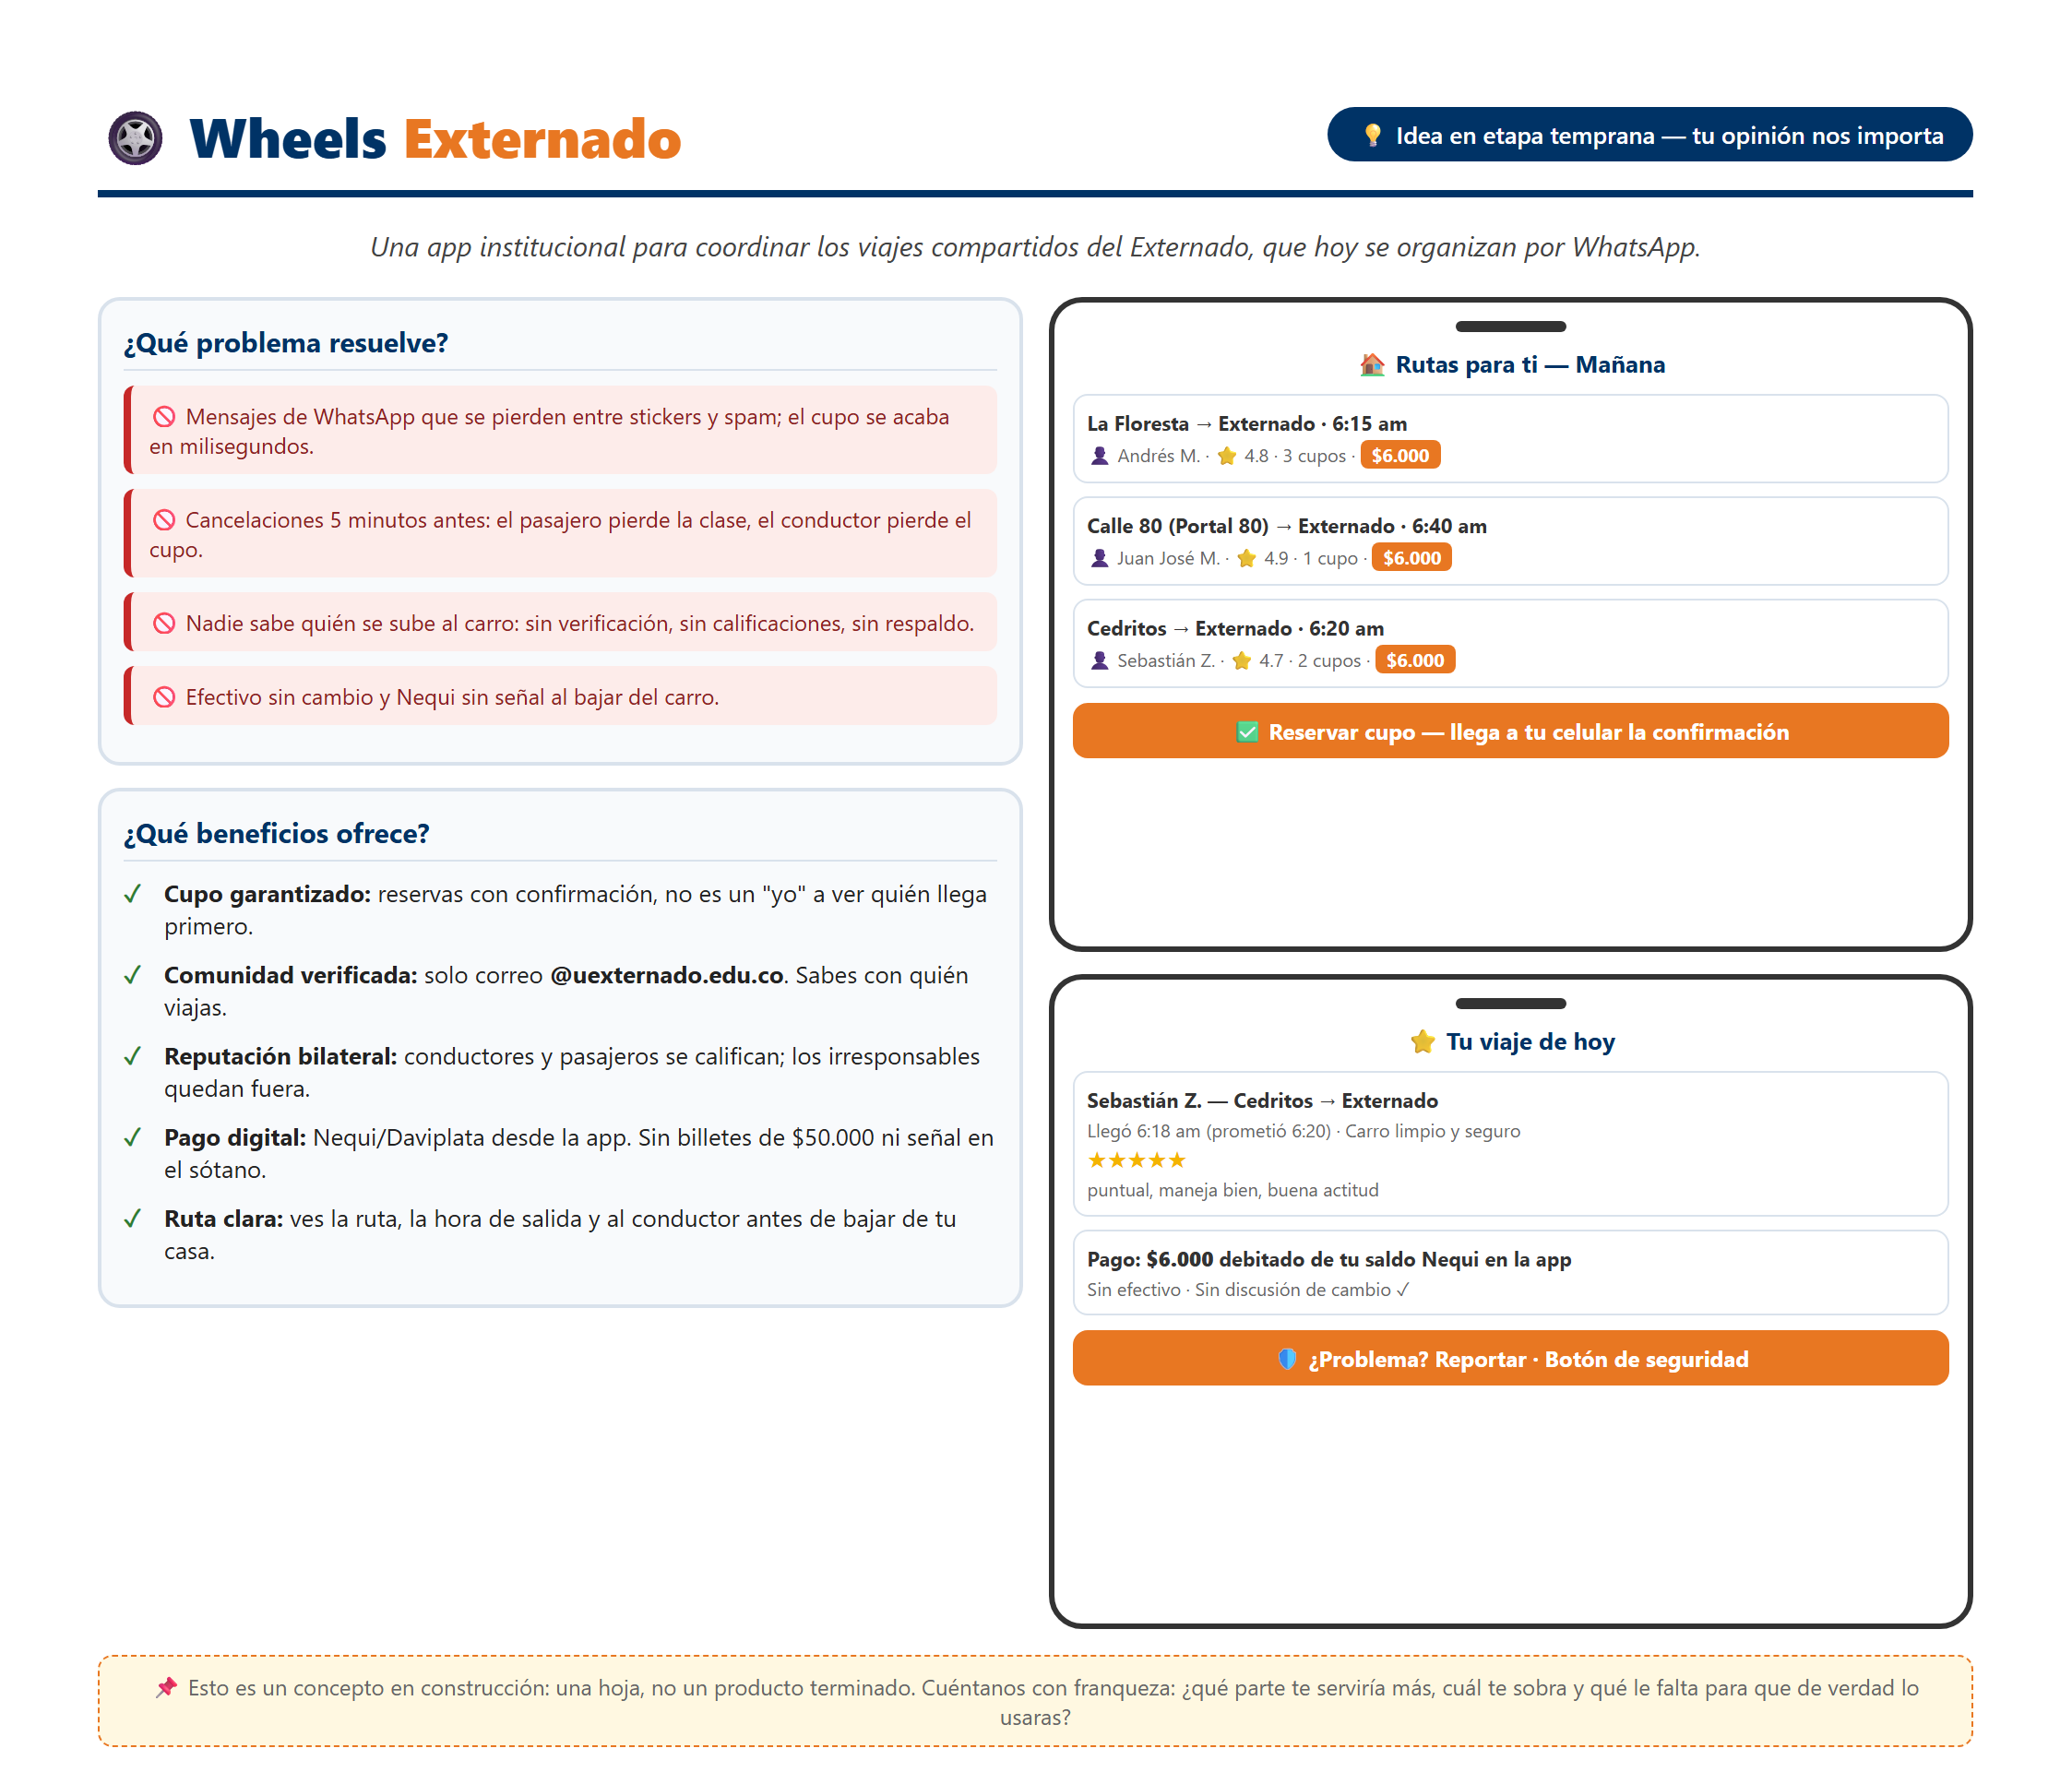
\includegraphics[width=0.74\textwidth]{Concepto_Wheels.png}
    \caption{L\'amina conceptual de Wheels Externado exhibida a los clientes durante el Customer Discovery.}
    \label{fig:concepto_wheels}
\end{figure}

\subsection{Desglose de los Componentes Funcionales Evaluados en Campo}
\begin{enumerate}[leftmargin=*]
    \item \textbf{Pantalla 1 --- B\'usqueda y Reserva Anticipada de Cupos:} Permite al pasajero programar y asegurar su viaje desde la noche anterior filtrando por hora de llegada al campus (7:00 a.m., 9:00 a.m.), facultad y corredor de origen. Los 4 informantes destacaron que esto elimina la ansiedad y la p\'erdida de tiempo de WhatsApp.
    \item \textbf{Pantalla 2 --- M\'odulo de Seguridad \guillemotleft Rutas Solo Chicas\guillemotright:} Filtro opcional que restringe la visualizaci\'on y abordaje exclusivamente a conductoras y pasajeras verificadas. Altamente ponderado por las informantes femeninas (E9 y E11) como una innovaci\'on ausente en Uber o InDrive.
    \item \textbf{Pantalla 3 --- Billetera y Liquidaci\'on Digital:} Pasarela transparente que debita \$8.000 COP al pasajero, transfiere \$6.800 COP directos a la cuenta Nequi/Daviplata del conductor al culminar el trayecto y retiene \$1.200 COP de comisi\'on de servicio. Ambos conductores (E11 y E12) validaron que este esquema evita cobros en efectivo y garantiza el dinero.
    \item \textbf{Pantalla 4 --- Verificaci\'on Institucional y Reputaci\'on:} Acceso restringido \'unicamente con credenciales institucionales \texttt{@uexternado.edu.co}, visualizaci\'on de placa del autom\'ovil, fotograf\'ia y calificaci\'on bilateral hist\'orica.
\end{enumerate}

\section{Base de Datos del Trabajo de Campo (E1 a E12)}

Conforme a las exigencias de la gu\'ia y del marco de dos lados de la plataforma, la base de datos se desglosa en los dos arquetipos analizados:

\subsection{Tabla D.1: Muestra de Pasajeros (Demanda --- $n=8$)}
\begin{table}[!htbp]
\centering
\scriptsize
\setlength{\tabcolsep}{3pt}
\renewcommand{\arraystretch}{1.15}
\begin{tabularx}{\textwidth}{c>{\bfseries}p{1.3cm}p{1.9cm}p{1.6cm}p{1.8cm}p{2.6cm}X}
\toprule
C\'od. & Carrera & Procedencia & Frecuencia & Gasto / WTP & Soluci\'on Actual & Cita Clave \\
\midrule
E1 & Derecho (8.\textsuperscript{vo}) & La Floresta / Cll 80 & Habitual (4 d/sem) & \$6.000 / hasta \$8.000 & WhatsApp Externado & \guillemotleft Es una loter\'ia responder 'yo' a tiempo.\guillemotright \\
\midrule
E2 & C. Datos (4.\textsuperscript{to}) & Facatativ\'a / Cll 13 & Diario (5 d/sem) & \$6.000 / hasta \$10.000 & Flota intermunicipal y WhatsApp & \guillemotleft Ser\'ia la salvaci\'on... pagar\'ia hasta \$10.000.\guillemotright \\
\midrule
E3 & Adm. Emp. (6.\textsuperscript{to}) & Suba / Av. Boyac\'a & 3--4 veces/sem & \$5.000--\$6.000 & Chats de WhatsApp & \guillemotleft Te toca leer 400 mensajes para encontrar una ruta.\guillemotright \\
\midrule
E4 & Enfermer\'ia (5.\textsuperscript{to}) & Bosa / AutoSur & 3 d\'ias/sem & \$6.000 (Uber: \$30k) & Grupos de WhatsApp & \guillemotleft Terminas tomando Uber de af\'an pagando \$30.000.\guillemotright \\
\midrule
E6 & Derecho (2.\textsuperscript{do}) & San Crist\'obal Sur & Diario & \$6.000 / hasta \$15.000 & SITP y Wheels de conocidos & \guillemotleft Duermo apenas cuatro horas por el transporte.\guillemotright \\
\midrule
E8 & Comunic. (3.\textsuperscript{er}) & Colina Campestre & Tardes/Noches & \$5.000--\$6.000 & Grupos de WhatsApp & \guillemotleft Al conductor se le notaba aliento alcoh\'olico.\guillemotright \\
\midrule
E9 & Derecho (6.\textsuperscript{to}) & Timiza / Kennedy & Diario (pr\'acticas) & \$6.000 / hasta \$8.000 & Chats de WhatsApp & \guillemotleft Uno revisa la placa y se la manda a la mam\'a.\guillemotright \\
\midrule
E10 & Ing. Ind. (4.\textsuperscript{to}) & Chapinero / Cll 67 & 3 veces/sem & \$6.000 / hasta \$7.000 & Chats de WhatsApp & \guillemotleft Leer 400 mensajes es perder toda la ma\~nana.\guillemotright \\
\bottomrule
\end{tabularx}
\caption{Base de datos anonimizada de informantes: Pasajeros (Demanda).}
\label{tab:base_pasajeros}
\end{table}

\subsection{Tabla D.2: Muestra de Conductores (Oferta --- $n=4$)}
\begin{table}[!htbp]
\centering
\scriptsize
\setlength{\tabcolsep}{3pt}
\renewcommand{\arraystretch}{1.15}
\begin{tabularx}{\textwidth}{c>{\bfseries}p{1.3cm}p{1.9cm}p{1.6cm}p{1.8cm}p{2.6cm}X}
\toprule
C\'od. & Carrera & Procedencia & Cupos Ofrecidos & Recaudo Diario & Dolor Cr\'itico del Conductor & Cita Clave \\
\midrule
E5 & Econom\'ia (7.\textsuperscript{mo}) & Cedritos / AutoNorte & 3 cupos (\$6.000) & \$18.000 COP & \textit{Ghosting}: cancelan a 5 min de salida; parqueadero \$22k & \guillemotleft El mensaje se pierde... me cancelan 5 min antes.\guillemotright \\
\midrule
E7 & C. Datos (5.\textsuperscript{to}) & Salitre / Cll 26 & 4 cupos (\$6.000) & \$24.000 COP & Dinero de reserva no asegurado; coordinaci\'on manual & \guillemotleft Me dejan colgado con el puesto y la gasolina corre.\guillemotright \\
\midrule
E11 & Derecho (8.\textsuperscript{vo}) & Portal Sur & 3 cupos fijados & \$18.000 COP & Quiere pago digital inmediato sin retenci\'on; viaje seguro mujeres & \guillemotleft Si el pago no me llega al terminar, vuelvo a WhatsApp.\guillemotright \\
\midrule
E12 & Derecho (4.\textsuperscript{to}) & Fontib\'on / Cll 26 & 4 cupos (\$6.000) & \$24.000 COP & Falta de compromiso de pasajeros; viajes vac\'ios & \guillemotleft Me cancelan a \'ultima hora y viajo con dos cupos vac\'ios.\guillemotright \\
\bottomrule
\end{tabularx}
\caption{Base de datos anonimizada de informantes: Conductores (Oferta).}
\label{tab:base_conductores}
\end{table}

\section{Evidencias de Consentimiento y Compromisos para Campo 3}

\subsection{E.1 Registro y Custodia del Consentimiento Informado}
\begin{table}[!htbp]
\centering
\small
\renewcommand{\arraystretch}{1.15}
\begin{tabularx}{\textwidth}{p{3.2cm}p{5.5cm}X}
\toprule
\textbf{C\'odigos de Informante} & \textbf{M\'etodo de Registro de Consentimiento} & \textbf{Soporte y Ubicaci\'on de Custodia} \\
\midrule
\textbf{E9, E10, E11, E12} & Lectura del protocolo institucional y autorizaci\'on expl\'icita verbal grabada al inicio de la sesi\'on. & Archivos de audio digital archivados en la carpeta segura de investigaci\'on del equipo (\texttt{Audios/}). \\
\midrule
\textbf{E1 a E8} & Consentimiento verbal informado al inicio de la entrevista presencial; ratificaci\'on y confirmaci\'on posterior v\'ia mensaje digital de WhatsApp. & Capturas de pantalla de confirmaci\'on de participaci\'on voluntaria archivadas en el repositorio seguro. \\
\bottomrule
\end{tabularx}
\caption{Matriz de registro y auditor\'ia del consentimiento informado.}
\label{tab:evidencias_consentimiento}
\end{table}

\subsection{E.2 Compromisos Concretados para el Trabajo de Campo 3 (User Testing)}
La gu\'ia de la c\'atedra exige evidenciar compromisos reales que trasciendan la intenci\'on verbal. Durante las entrevistas E9 a E12 se obtuvieron \textbf{4 compromisos firmes de prueba} y \textbf{4 contactos referidos directos}:

\begin{table}[!htbp]
\centering
\small
\renewcommand{\arraystretch}{1.15}
\begin{tabularx}{\textwidth}{cl X p{4.2cm}}
\toprule
\textbf{C\'od.} & \textbf{Rol} & \textbf{Compromiso Asumido para Campo 3} & \textbf{Canal y Corredor Acordado} \\
\midrule
\textbf{E9} & Pasajera & Acept\'o formalmente probar el prototipo de usuario navegable y validar el filtro de \guillemotleft Solo Chicas\guillemotright; aport\'o 1 referido directo. & WhatsApp / Corredor Timiza (Kennedy). \\
\midrule
\textbf{E10} & Pasajero & Acept\'o evaluar los flujos de b\'usqueda, reserva anticipada y pago digital en el prototipo; aport\'o 1 referido. & WhatsApp / Corredor Chapinero y Suba. \\
\midrule
\textbf{E11} & Conductora & Acept\'o probar el m\'odulo de conductor, publicaci\'on de ruta y liquidaci\'on en cuenta de billetera m\'ovil; aport\'o 1 referida. & WhatsApp / Corredor Portal Sur y Am\'ericas. \\
\midrule
\textbf{E12} & Conductor & Acept\'o testear la pol\'itica de abonos de reserva y penalizaci\'on por \textit{ghosting} en sus trayectos; aport\'o 1 referido. & WhatsApp / Corredor Calle 26 y Fontib\'on. \\
\bottomrule
\end{tabularx}
\caption{Matriz de compromisos concretados y contactos para el Trabajo de Campo 3.}
\label{tab:compromisos_campo3}
\end{table}

\section{Declaraciones \'Eticas y Cumplimiento Normativo}

\subsection{F.1 Declaraci\'on de No Participaci\'on de Menores de Edad}
El equipo deja constancia expresa de que el 100\% de los informantes que participaron en las 12 entrevistas semiestructuradas (E1 a E12) corresponden a estudiantes legalmente mayores de edad (entre 18 y 25 a\~nos), con plena capacidad jur\'idica para otorgar su consentimiento informado aut\'onomo. No se requiri\'o autorizaci\'on de tutores legales ni representantes de menores.

\subsection{F.2 Declaraci\'on Sobre Observaci\'on Pasiva Invasiva}
De conformidad con los l\'imites metodol\'ogicos de la investigaci\'on cualitativa primaria, no se realiz\'o observaci\'on encubierta, filmaci\'on en v\'ia p\'ublica ni intervenci\'on invasiva en autom\'oviles privados. Todas las observaciones correspondieron al registro libre de din\'amicas de interacci\'on dentro de los grupos comunitarios p\'ublicos de WhatsApp de los cuales los fundadores forman parte leg\'itima como estudiantes.

\subsection{F.3 Cumplimiento de la Ley Estatutaria 1581 de 2012 de Protecci\'on de Datos}
En estricto apego a la legislaci\'on colombiana de Habeas Data (Ley 1581 de 2012 y Decreto Reglamentario 1377 de 2013), todos los nombres propios, n\'umeros de tel\'efono y datos sensibles de los participantes fueron disociados de los informes entregables, custodiando las grabaciones en servidores con autenticaci\'on de doble factor exclusiva para los integrantes del Grupo 5. La informaci\'on recopilada ser\'a destruida una vez culminada la evaluaci\'on formal de la c\'atedra.

\end{document}
